\documentclass[10pt]{article}
\usepackage[T1]{fontenc}
\usepackage[utf8]{inputenc}
%\DeclareUnicodeCharacter{00A0}{ }
%\usepackage[adobe-utopia]{mathdesign}

\usepackage{amsmath}
\usepackage[francais]{babel}
\usepackage[dvips]{graphicx}
%\usepackage{here}
\usepackage{framed}
\usepackage[normalem]{ulem}
\usepackage{fancyhdr}
\usepackage{titlesec}
\usepackage{vmargin}

\usepackage{amsmath}
\usepackage{ifthen}
\usepackage{multirow}
\usepackage{multicol} % Portions de texte en colonnes

%\usepackage{xltxtra} % Logo XeLaTeX
%\usepackage{pst-solides3d}
\usepackage{color}
%\usepackage{colortbl}
\usepackage{titletoc} % Pour la mise en forme de la table des matières

%\usepackage[crop=off]{auto-pst-pdf}
%\usepackage{bclogo}


%\usepackage{longtable}
%\usepackage{flafter}%floatants après la référence
%\usepackage{pst-solides3d}
%\usepackage{pstricks}
%\usepackage{minitoc}
%\setcounter{minitocdepth}{4}
%\usepackage{draftcopy}% "Brouillon"
%\usepackage{floatflt}
%\usepackage{psfrag}
%\usepackage{listings} % Permet d'insérer du code de programmation
%\usepackage{lmodern}
%\usepackage[adobe-utopia,uppercase=upright,greeklowercase=upright]{mathdesign}
%\usepackage{minionpro}
%\usepackage{pifont}
%\usepackage{amssymb}
%\usepackage[francais]{varioref}

\setmarginsrb{1.5cm}{1cm}{1cm}{1.5cm}{1cm}{1cm}{1cm}{1cm}

\definecolor{gris25}{gray}{0.75}
\definecolor{bleu}{RGB}{18,33,98}
\definecolor{bleuf}{RGB}{42,94,171}
\definecolor{bleuc}{RGB}{231,239,247}
\definecolor{rougef}{RGB}{185,18,27}
\definecolor{rougec}{RGB}{255,230,231}
\definecolor{vertf}{RGB}{103,126,82}
\definecolor{vertc}{RGB}{220,255,191}
\definecolor{violetf}{RGB}{112,48,160}
\definecolor{violetc}{RGB}{230,224,236}
\definecolor{jaunec}{RGB}{220,255,191}
%\usepackage{algorithm}
%\usepackage{algorithmic}
\usepackage[french]{algorithm2e}

\SetKwBlock{Fonction}{Début Fonction}{Fin Fonction}
\SetKwComment{Comment}{start}{end}
% Python sources

\usepackage{listings}
\lstloadlanguages{R}   % pour regler les pb d accent utf8 dans les codes
\lstset{language=R} % pour regler les pb d accent utf8 dans les codes

\usepackage{textcomp}
\usepackage{setspace}
%\usepackage{palatino}

%\usepackage{color}
\definecolor{Bleu}{rgb}{0.1,0.1,1.0}
\definecolor{Noir}{rgb}{0,0,0}
\definecolor{Grau}{rgb}{0.5,0.5,0.5}
\definecolor{DunkelGrau}{rgb}{0.15,0.15,0.15}
\definecolor{Hellbraun}{rgb}{0.5,0.25,0.0}
\definecolor{Magenta}{rgb}{1.0,0.0,1.0}
\definecolor{Gris}{gray}{0.5}
\definecolor{Vert}{rgb}{0,0.5,0}
\definecolor{SourceHintergrund}{rgb}{1,1.0,0.95}


%
\renewcommand{\lstlistlistingname}{Listings}
\renewcommand{\lstlistingname}{Listing}

\lstnewenvironment{python}[1][]{
\lstset{
%escapeinside={\%*}{*)},
%inputencoding=utf8,   % pour regler les pb d accent utf8 dans les codes
%extendedchars=true,   % pour regler les pb d accent utf8 dans les codes
language=python,
basicstyle=\sffamily\footnotesize, 	
stringstyle=\color{red}, 
showstringspaces=false, 
alsoletter={1234567890},
otherkeywords={\ , \}, \{},
keywordstyle=\color{blue},
emph={access,and,break,class,continue,def,del,elif ,else,
except,exec,finally,for,from,global,if,import,in,i s,
lambda,not,or,pass,print,raise,return,try,while},
emphstyle=\color{black}\bfseries,
emph={[2]True, False, None, self},
emphstyle=[2]\color{olive},
emph={[3]from, import, as},
emphstyle=[3]\color{blue},
upquote=true,
columns=flexible, % pour empecher d'avoir un espacement mono
morecomment=[s]{"""}{"""},
commentstyle=\color{Hellbraun}\slshape, 
%emph={[4]1, 2, 3, 4, 5, 6, 7, 8, 9, 0},
emphstyle=[4]\color{blue},
literate=*{:}{{\textcolor{blue}:}}{1}
{=}{{\textcolor{blue}=}}{1}
{-}{{\textcolor{blue}-}}{1}
{+}{{\textcolor{blue}+}}{1}
{*}{{\textcolor{blue}*}}{1}
{!}{{\textcolor{blue}!}}{1}
{(}{{\textcolor{blue}(}}{1}
{)}{{\textcolor{blue})}}{1}
{[}{{\textcolor{blue}[}}{1}
{]}{{\textcolor{blue}]}}{1}
{<}{{\textcolor{blue}<}}{1}
{>}{{\textcolor{blue}>}}{1}
{COMPLETER}{{\textcolor{red}COMPLETER}}{1},
literate=%
            {é}{{\'{e}}}1
            {è}{{\`{e}}}1
            {ê}{{\^{e}}}1
            {ë}{{\¨{e}}}1
            {û}{{\^{u}}}1
            {ù}{{\`{u}}}1
            {â}{{\^{a}}}1
            {à}{{\`{a}}}1
            {î}{{\^{i}}}1
            {ç}{{\c{c}}}1
            {Ç}{{\c{C}}}1
            {É}{{\'{E}}}1
            {Ê}{{\^{E}}}1
            {À}{{\`{A}}}1
            {Â}{{\^{A}}}1
            {Î}{{\^{I}}}1, % pour regler les pb d accent utf8 dans les codes
%framexleftmargin=1mm, framextopmargin=1mm, frame=shadowbox, rulesepcolor=\color{blue},#1
%backgroundcolor=\color{SourceHintergrund}, 
%framexleftmargin=1mm, framexrightmargin=1mm, framextopmargin=1mm, frame=single, framerule=1pt, rulecolor=\color{black},#1
}}{}



\lstnewenvironment{scilab}[1][]{
\lstset{
language=scilab,
basicstyle=\sffamily\footnotesize, 	
stringstyle=\color{red}, 
showstringspaces=false, 
alsoletter={1234567890},
otherkeywords={\ , \}, \{},
keywordstyle=\color{blue},
emph={access,and,break,class,continue,def,del,elif ,else,
except,exec,finally,for,from,global,if,import,in,i s,
lambda,not,or,pass,print,raise,return,try,while,Debut},
emphstyle=\color{black}\bfseries,
emph={[2]True, False, None, self},
emphstyle=[2]\color{olive},
emph={[3]from, import, as},
emphstyle=[3]\color{blue},
upquote=true,
columns=flexible, % pour empecher d'avoir un espacement mono
morecomment=[s]{"""}{"""},
commentstyle=\color{Hellbraun}\slshape, 
%emph={[4]1, 2, 3, 4, 5, 6, 7, 8, 9, 0},
emphstyle=[4]\color{blue},
literate=*{:}{{\textcolor{blue}:}}{1}
{=}{{\textcolor{blue}=}}{1}
{-}{{\textcolor{blue}-}}{1}
{+}{{\textcolor{blue}+}}{1}
{*}{{\textcolor{blue}*}}{1}
{!}{{\textcolor{blue}!}}{1}
{(}{{\textcolor{blue}(}}{1}
{)}{{\textcolor{blue})}}{1}
{[}{{\textcolor{blue}[}}{1}
{]}{{\textcolor{blue}]}}{1}
{<}{{\textcolor{blue}<}}{1}
{>}{{\textcolor{blue}>}}{1},
%framexleftmargin=1mm, framextopmargin=1mm, frame=shadowbox, rulesepcolor=\color{blue},#1
%backgroundcolor=\color{SourceHintergrund}, 
%framexleftmargin=1mm, framexrightmargin=1mm, framextopmargin=1mm, frame=single, framerule=1pt, rulecolor=\color{black},#1
}}{}


\lstdefinestyle{stylepython}{%
escapeinside={\%*}{*)},
inputencoding=utf8,   % pour regler les pb d accent utf8 dans les codes
extendedchars=true,   % pour regler les pb d accent utf8 dans les codes
language=python,
basicstyle=\sffamily\footnotesize, 	
stringstyle=\color{red}, 
showstringspaces=false, 
alsoletter={1234567890},
otherkeywords={\ , \}, \{},
keywordstyle=\color{blue},
emph={access,and,break,class,continue,def,del,elif ,else,
except,exec,finally,for,from,global,if,import,in,i s,
lambda,not,or,pass,print,raise,return,try,while},
emphstyle=\color{black}\bfseries,
emph={[2]True, False, None, self},
emphstyle=[2]\color{green},
emph={[3]from, import, as},
emphstyle=[3]\color{blue},
upquote=true,
columns=flexible, % pour empecher d'avoir un espacement mono
morecomment=[s]{"""}{"""},
commentstyle=\color{Hellbraun}\slshape, 
%emph={[4]1, 2, 3, 4, 5, 6, 7, 8, 9, 0},
emphstyle=[4]\color{blue},
literate=*{:}{{\textcolor{blue}:}}{1}
{=}{{\textcolor{blue}=}}{1}
{-}{{\textcolor{blue}-}}{1}
{+}{{\textcolor{blue}+}}{1}
{*}{{\textcolor{blue}*}}{1}
{!}{{\textcolor{blue}!}}{1}
{(}{{\textcolor{blue}(}}{1}
{)}{{\textcolor{blue})}}{1}
{[}{{\textcolor{blue}[}}{1}
{]}{{\textcolor{blue}]}}{1}
{<}{{\textcolor{blue}<}}{1}
{>}{{\textcolor{blue}>}}{1}
{COMPLETER}{{\textcolor{red}COMPLETER}}{1},
literate=%
            {é}{{\'{e}}}1
            {è}{{\`{e}}}1
            {ê}{{\^{e}}}1
            {ë}{{\¨{e}}}1
            {û}{{\^{u}}}1
            {ù}{{\`{u}}}1
            {â}{{\^{a}}}1
            {à}{{\`{a}}}1
            {î}{{\^{i}}}1
            {ç}{{\c{c}}}1
            {Ç}{{\c{C}}}1
            {É}{{\'{E}}}1
            {Ê}{{\^{E}}}1
            {À}{{\`{A}}}1
            {Â}{{\^{A}}}1
            {Î}{{\^{I}}}1,
%numbers=left,                    % where to put the line-numbers; possible values are (none, left, right)
%numbersep=5pt,                   % how far the line-numbers are from the code
%numberstyle=\tiny\color{mygray}, % the style that is used for the line-numbers
}

%
%\renewcommand{\algorithmicrequire} {\textbf{\textsc{Entrées:}}}
%\renewcommand{\algorithmicensure}  {\textbf{\textsc{Sorties:}}}
%\renewcommand{\algorithmicwhile}   {\textbf{tantque}}
%\renewcommand{\algorithmicdo}      {\textbf{faire}}
%\renewcommand{\algorithmicendwhile}{\textbf{fin tantque}}
%\renewcommand{\algorithmicend}     {\textbf{fin}}
%\renewcommand{\algorithmicif}      {\textbf{si}}
%\renewcommand{\algorithmicendif}   {\textbf{finsi}}
%\renewcommand{\algorithmicelse}    {\textbf{sinon}}
%\renewcommand{\algorithmicthen}    {\textbf{alors}}
%\renewcommand{\algorithmicfor}     {\textbf{pour}}
%\renewcommand{\algorithmicforall}  {\textbf{pour tout}}
%\renewcommand{\algorithmicdo}      {\textbf{faire}}
%\renewcommand{\algorithmicendfor}  {\textbf{fin pour}}
%\renewcommand{\algorithmicloop}    {\textbf{boucler}}
%\renewcommand{\algorithmicendloop} {\textbf{fin boucle}}
%\renewcommand{\algorithmicrepeat}  {\textbf{répéter}}
%\renewcommand{\algorithmicuntil}   {\textbf{jusqu'à}}

\lstnewenvironment{termi}[1][]{
\lstset{
language=scilab,
basicstyle=\sffamily\footnotesize, 	
stringstyle=\color{red}, 
showstringspaces=false, 
alsoletter={1234567890},
otherkeywords={\ , \}, \{},
keywordstyle=\color{blue},
emph={access,and,break,class,continue,def,del,elif ,else,
except,exec,finally,for,from,global,if,import,in,i s,
lambda,not,or,pass,print,raise,return,try,while,Debut},
emphstyle=\color{black}\bfseries,
emph={[2]True, False, None, self},
emphstyle=[2]\color{green},
emph={[3]from, import, as},
emphstyle=[3]\color{blue},
upquote=true,
columns=flexible, % pour empecher d'avoir un espacement mono
morecomment=[s]{"""}{"""},
commentstyle=\color{Hellbraun}\slshape, 
%emph={[4]1, 2, 3, 4, 5, 6, 7, 8, 9, 0},
emphstyle=[4]\color{blue},
literate=*{:}{{\textcolor{blue}:}}{1}
{=}{{\textcolor{blue}=}}{1}
{-}{{\textcolor{blue}-}}{1}
{+}{{\textcolor{blue}+}}{1}
{*}{{\textcolor{blue}*}}{1}
{!}{{\textcolor{blue}!}}{1}
{(}{{\textcolor{blue}(}}{1}
{)}{{\textcolor{blue})}}{1}
{[}{{\textcolor{blue}[}}{1}
{]}{{\textcolor{blue}]}}{1}
{<}{{\textcolor{blue}<}}{1}
{>}{{\textcolor{blue}>}}{1},
%framexleftmargin=1mm, framextopmargin=1mm, frame=shadowbox, rulesepcolor=\color{blue},#1
%backgroundcolor=\color{SourceHintergrund}, 
%framexleftmargin=1mm, framexrightmargin=1mm, framextopmargin=1mm, frame=single, framerule=1pt, rulecolor=\color{black},#1
}}{}


%
%\renewcommand{\algorithmicrequire} {\textbf{\textsc{Entrées:}}}
%\renewcommand{\algorithmicensure}  {\textbf{\textsc{Sorties:}}}
%\renewcommand{\algorithmicwhile}   {\textbf{tantque}}
%\renewcommand{\algorithmicdo}      {\textbf{faire}}
%\renewcommand{\algorithmicendwhile}{\textbf{fin tantque}}
%\renewcommand{\algorithmicend}     {\textbf{fin}}
%\renewcommand{\algorithmicif}      {\textbf{si}}
%\renewcommand{\algorithmicendif}   {\textbf{finsi}}
%\renewcommand{\algorithmicelse}    {\textbf{sinon}}
%\renewcommand{\algorithmicthen}    {\textbf{alors}}
%\renewcommand{\algorithmicfor}     {\textbf{pour}}
%\renewcommand{\algorithmicforall}  {\textbf{pour tout}}
%\renewcommand{\algorithmicdo}      {\textbf{faire}}
%\renewcommand{\algorithmicendfor}  {\textbf{fin pour}}
%\renewcommand{\algorithmicloop}    {\textbf{boucler}}
%\renewcommand{\algorithmicendloop} {\textbf{fin boucle}}
%\renewcommand{\algorithmicrepeat}  {\textbf{répéter}}
%\renewcommand{\algorithmicuntil}   {\textbf{jusqu'à}}
%%%%%%%%%%%%
% Définition des vecteurs 
%%%%%%%%%%%%
 \newcommand{\vect}[1]{\overrightarrow{#1}}

%%%%%%%%%%%%
% Définition des torseurs 
%%%%%%%%%%%%

 \newcommand{\torseur}[1]{%
\left\{{#1}\right\}
}

\newcommand{\torseurcin}[3]{%
\left\{\mathcal{#1} \left(#2/#3 \right) \right\}
}

\newcommand{\torseurstat}[3]{%
\left\{\mathcal{#1} \left(#2\rightarrow #3 \right) \right\}
}

 \newcommand{\torseurc}[8]{%
%\left\{#1 \right\}=
\left\{
{#1}
\right\}
 = 
\left\{%
\begin{array}{cc}%
{#2} & {#5}\\%
{#3} & {#6}\\%
{#4} & {#7}\\%
\end{array}%
\right\}_{#8}%
}

 \newcommand{\torseurcol}[7]{
\left\{%
\begin{array}{cc}%
{#1} & {#4}\\%
{#2} & {#5}\\%
{#3} & {#6}\\%
\end{array}%
\right\}_{#7}%
}

 \newcommand{\torseurl}[3]{%
%\left\{\mathcal{#1}\right\}_{#2}=%
\left\{%
\begin{array}{l}%
{#1} \\%
{#2} %
\end{array}%
\right\}_{#3}%
}

 \newcommand{\vectv}[3]{%
\vect{V\left( {#1} \in {#2}/{#3}\right)}
}


\newcommand{\vectf}[2]{%
\vect{R\left( {#1} \rightarrow {#2}\right)}
}

\newcommand{\vectm}[3]{%
\vect{\mathcal{M}\left( {#1}, {#2} \rightarrow {#3}\right)}
}


 \newcommand{\vectg}[3]{%
\vect{\Gamma \left( {#1} \in {#2}/{#3}\right)}
}

 \newcommand{\vecto}[2]{%
\vect{\Omega\left( {#1}/{#2}\right)}
}
% }$$\left\{\mathcal{#1} \right\}_{#2} =%
% \left\{%
% \begin{array}{c}%
%  #3 \\%
%  #4 %
% \end{array}%
% \right\}_{#5}}
\setcounter{tocdepth}{2}
% \mtcselectlanguage{french} 


%  ------------------------------------------
% | Modification du formatage des sections : | 
%  ------------------------------------------

% Grands titres :
% ---------------

\newcommand{\titre}[1]{%
\begin{center}
      \bigskip
      \rule{\textwidth}{1pt}
      \par\vspace{0.1cm}
      
      \textbf{\large #1}
      \par\rule{\textwidth}{1pt}
    \end{center}
    \bigskip
  }

% Supprime le numéro du chapitre dans la numérotation des sections:
% -----------------------------------------------------------------
\makeatletter
\renewcommand{\thesection}{\@arabic\c@section}
\makeatother


% \titleformat{\chapter}[display]
% {\normalfont\Large\filcenter}
% {}
% {1pc}
% {\titlerule[1pt]
%   \vspace{1pc}%
%   \Huge}[\vspace{1ex}%
% \titlerule]


%%%% Chapitres Comme PY Pechard %%%%%%%%%
% numéro du chapitre
\DeclareFixedFont{\chapnumfont}{OT1}{phv}{b}{n}{80pt}
% pour le mot « Chapitre »
\DeclareFixedFont{\chapchapfont}{OT1}{phv}{m}{it}{40pt}
% pour le titre
\DeclareFixedFont{\chaptitfont}{T1}{phv}{b}{n}{25pt}

\definecolor{gris}{gray}{0.75}
\titleformat{\chapter}[display]%
	{\sffamily}%
	{\filleft\chapchapfont\color{gris}\chaptertitlename\
	\\
	\vspace{12pt}
	\chapnumfont\thechapter}%
	{16pt}%
	{\filleft\chaptitfont}%
	[\vspace{6pt}\titlerule\titlerule\titlerule]

%%%%  Fin Chapitres Comme PY Pechard %%%%%%%%%


% Section, subsection, subsubsection sans serifs :
% % ----------------------------------------------

% \makeatletter
% \renewcommand{\section}{\@startsection{section}{0}{0mm}%
% {\baselineskip}{.3\baselineskip}%
% {\normalfont\sffamily\Large\textbf}}%
% \makeatother

\makeatletter
\renewcommand{\@seccntformat}[1]{{\textcolor{bleu}{\csname
the#1\endcsname}\hspace{0.5em}}}
\makeatother

\makeatletter
\renewcommand{\section}{\@startsection{section}{1}{\z@}%
                       {-4ex \@plus -1ex \@minus -.4ex}%
                       {1ex \@plus.2ex }%
                       {\normalfont\Large\sffamily\bfseries}}%
\makeatother
 
\makeatletter
\renewcommand{\subsection}{\@startsection {subsection}{2}{\z@}
                          {-3ex \@plus -0.1ex \@minus -.4ex}%
                          {0.5ex \@plus.2ex }%
                          {\normalfont\large\sffamily\bfseries}}
\makeatother
 
\makeatletter
\renewcommand{\subsubsection}{\@startsection {subsubsection}{3}{\z@}
                          {-2ex \@plus -0.1ex \@minus -.2ex}%
                          {0.2ex \@plus.2ex }%
                          {\normalfont\large\sffamily\bfseries}}
\makeatother
 
\makeatletter             
\renewcommand{\paragraph}{\@startsection{paragraph}{4}{\z@}%
                                    {-2ex \@plus-.2ex \@minus .2ex}%
                                    {0.1ex}%               
{\normalfont\sffamily\bfseries}}
\makeatother
 
 
\makeatletter             
\renewcommand{\subparagraph}{\@startsection{subparagraph}{5}{\z@}%
                                    {-2ex \@plus-.2ex \@minus .2ex}%
                                    {0ex}%               
{\normalfont\bfseries Question }}
\makeatother
\renewcommand{\thesubparagraph}{\arabic{subparagraph}} 
\makeatletter

\setcounter{secnumdepth}{5}





% Formatage de la table des matières 
% Paquets nécessaires : titletoc ?

% Chapitre spéciaux écrits dans un nombre cerclé dans la table des matières.
\titlecontents{chapter}[+3pc]
  {\addvspace{10pt}\sffamily\bfseries}
{\contentslabel[{\pscirclebox[fillstyle=solid,fillcolor=gray!25,
linecolor=gray!25,framesep=4pt]{\textcolor{white}{\thecontentslabel}}}]{2.5pc}}
  {}
  {\dotfill \normalfont\thecontentspage\ }

\titlecontents{section}[3pc]
  {\addvspace{2pt}\sffamily}
  {\contentslabel[\thecontentslabel]{1.8pc}}
  {}
  {\dotfill \normalfont\thecontentspage\ }

\titlecontents{subsection}[5pc]
  {\addvspace{2pt}\sffamily}
  {\contentslabel[\thecontentslabel]{1.8pc}}
  {}
  {\dotfill \normalfont\thecontentspage\ }

\titlecontents{subsubsection}[8pc]
  {\addvspace{2pt}\sffamily}
  {\contentslabel[\thecontentslabel]{3pc}}
  {}
  {\dotfill \normalfont\thecontentspage\ }
%{\;\titlerule\;\normalfont\thecontentspage\ }

\titlecontents{paragraph}[9pc]
  {\addvspace{2pt}\sffamily}
  {\contentslabel[\thecontentslabel]{3.5pc}}
  {}
  {\dotfill \normalfont\thecontentspage\ }

%pour avoir l indentation dans minipage
\newdimen\oldparindent\oldparindent=\parindent

\makeatletter
\def\@iiiminipage#1#2[#3]#4{%
  \noindent
  \leavevmode
  \@pboxswfalse
  \setlength\@tempdima{#4}%
  \def\@mpargs{{#1}{#2}[#3]{#4}}%
  \setbox\@tempboxa\vbox\bgroup
    \color@begingroup
      \hsize\@tempdima
      \textwidth\hsize \columnwidth\hsize
      \@parboxrestore
      \parindent=\oldparindent
      \def\@mpfn{mpfootnote}\def\thempfn{\thempfootnote}\c@mpfootnote\z@
      \let\@footnotetext\@mpfootnotetext
      \let\@listdepth\@mplistdepth \@mplistdepth\z@
      \@minipagerestore
      \@setminipage}
\makeatother

% Paquets requis : 

\definecolor{gris25}{gray}{0.75}
\definecolor{bleu}{RGB}{18,33,98}
\definecolor{bleuf}{RGB}{42,94,171}
\definecolor{bleuc}{RGB}{231,239,247}
\definecolor{rougef}{RGB}{185,18,27}
\definecolor{rougec}{RGB}{255,230,231}
\definecolor{vertf}{RGB}{103,126,82}
\definecolor{vertc}{RGB}{220,255,191}
\definecolor{violetf}{RGB}{112,48,160}
\definecolor{violetc}{RGB}{230,224,236}
\definecolor{jaunec}{RGB}{220,255,191}



\newenvironment{corrige}[1][\hsize]%
{%
    \def\FrameCommand%
    {%
\rotatebox{90}{\textit{\textsf{Corrigé}}} 
        {\color{violetf}\vrule width 3pt}%
        \hspace{0pt}%must no space.
        \fboxsep=\FrameSep\colorbox{violetc}%
    }%
    \MakeFramed{\hsize #1 \advance\hsize-\width\FrameRestore}%
}%
{\endMakeFramed}%

\newenvironment{sci}[1][\hsize]%
{%
    \def\FrameCommand%
    {%
%\rotatebox{90}{\textit{\textsf{Scilab}}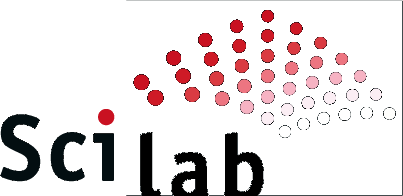
\includegraphics[height=.8cm]{png/logo_scilab}} 
\rotatebox{90}{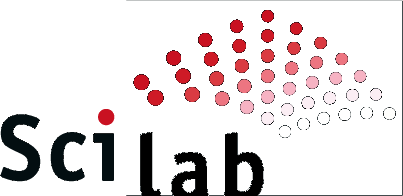
\includegraphics[height=.6cm]{png/logo_scilab}} 
        {\color{violetf}\vrule width 3pt}%
        \hspace{0pt}%must no space.
        \fboxsep=\FrameSep\colorbox{violetc}%
    }%
    \MakeFramed{\hsize #1 \advance\hsize-\width\FrameRestore}%
}%
{\endMakeFramed}%

\newenvironment{pseudo}[1][\hsize]%
{%
    \def\FrameCommand%
    {%
\rotatebox{90}{\textit{\textsf{Pseudo Code}}} 
        {\color{violetf}\vrule width 3pt}%
        \hspace{0pt}%must no space.
        \fboxsep=\FrameSep\colorbox{violetc}%
    }%
    \MakeFramed{\hsize #1 \advance\hsize-\width\FrameRestore}%
}%
{\endMakeFramed}%

\newenvironment{py}[1][\hsize]%
{%
    \def\FrameCommand%
    {%
%\rotatebox{90}{\textit{\textsf{Python}}} 
\rotatebox{90}{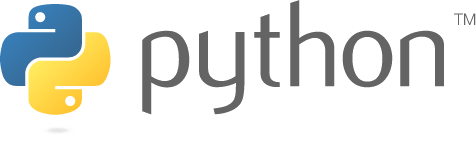
\includegraphics[height=.6cm]{png/logo_python}} 
        {\color{violetf}\vrule width 3pt}%
        \hspace{0pt}%must no space.
        \fboxsep=\FrameSep\colorbox{violetc}%
    }%
    \MakeFramed{\hsize #1 \advance\hsize-\width\FrameRestore}%
}%
{\endMakeFramed}%


\newenvironment{term}[1][\hsize]%
{%
    \def\FrameCommand%
    {%
\rotatebox{90}{\textit{\textsf{Terminal}}} 
        {\color{violetf}\vrule width 3pt}%
        \hspace{0pt}%must no space.
        \fboxsep=\FrameSep\colorbox{violetc}%
    }%
    \MakeFramed{\hsize #1 \advance\hsize-\width\FrameRestore}%
}%
{\endMakeFramed}%



\newenvironment{comp}[1][\hsize]%
{%
    \def\FrameCommand
    {%
\rotatebox{90}{\textit{\textsf{Compétences}}} 
        {\color{bleuf}\vrule width 3pt}%
        \hspace{0pt}%must no space.
        \fboxsep=\FrameSep\colorbox{bleuc}%
    }%
    \MakeFramed{\hsize#1\advance\hsize-\width\FrameRestore}%
}%
{\endMakeFramed}%

\newenvironment{rem}[1][\hsize]%
{%
    \def\FrameCommand
    {%
\rotatebox{90}{\textit{\textsf{Remarque}}} 
        {\color{bleuf}\vrule width 3pt}%
        \hspace{0pt}%must no space.
        \fboxsep=\FrameSep\colorbox{bleuc}%
    }%
    \MakeFramed{\hsize#1\advance\hsize-\width\FrameRestore}%
}%
{\endMakeFramed}%


\newenvironment{savoir}[1][\hsize]%
{%
    \def\FrameCommand
    {%
\rotatebox{90}{\textit{\textsf{Savoir}}} 
        {\color{bleuf}\vrule width 3pt}%
        \hspace{0pt}%must no space.
        \fboxsep=\FrameSep\colorbox{bleuc}%
    }%
    \MakeFramed{\hsize#1\advance\hsize-\width\FrameRestore}%
}%
{\endMakeFramed}%

\newenvironment{Objectif}[1][\hsize]%
{%
    \def\FrameCommand
    {%
\rotatebox{90}{\textit{\textsf{Objectif}}} 
        {\color{bleuf}\vrule width 3pt}%
        \hspace{0pt}%must no space.
        \fboxsep=\FrameSep\colorbox{bleuc}%
    }%
    \MakeFramed{\hsize#1\advance\hsize-\width\FrameRestore}%
}%
{\endMakeFramed}%

\newenvironment{prob}[1][\hsize]%
{%
    \def\FrameCommand%
    {%
\rotatebox{90}{\textit{\textsf{ Problématique}}} 
        {\color{rougef}\vrule width 3pt}%
        \hspace{0pt}%must no space.
        \fboxsep=\FrameSep\colorbox{rougec}%
    }%
    \MakeFramed{\hsize#1\advance\hsize-\width\FrameRestore}%
}%
{\endMakeFramed}%

\newenvironment{obj}[1][\hsize]%
{%
    \def\FrameCommand%
    {%
\rotatebox{90}{\textit{\textsf{Objectifs}}} 
        {\color{rougef}\vrule width 3pt}%
        \hspace{0pt}%must no space.
        \fboxsep=\FrameSep\colorbox{rougec}%
    }%
    \MakeFramed{\hsize#1\advance\hsize-\width\FrameRestore}%
}%
{\endMakeFramed}%

\newenvironment{defi}[1][\hsize]%
{%
    \def\FrameCommand%
    {%
\rotatebox{90}{\textit{\textsf{Définition\\}}} 
        {\color{bleuf}\vrule width 3pt}%
        \hspace{0pt}%must no space.
        \fboxsep=\FrameSep\colorbox{bleuc}%
    }%
    \MakeFramed{\hsize#1\advance\hsize-\width\FrameRestore}%
}%
{\endMakeFramed}%


\newenvironment{demo}[1][\hsize]%
{%
    \def\FrameCommand%
    {%
\rotatebox{90}{\textit{\textsf{Démonstration\\}}} 
        {\color{bleuf}\vrule width 3pt}%
        \hspace{0pt}%must no space.
        \fboxsep=\FrameSep\colorbox{bleuc}%
    }%
    \MakeFramed{\hsize#1\advance\hsize-\width\FrameRestore}%
}%
{\endMakeFramed}%


\newenvironment{hypo}[1][\hsize]%
{%
    \def\FrameCommand%
    {%
\rotatebox{90}{\textit{\textsf{Hypothèse\\}}} 
        {\color{bleuf}\vrule width 3pt}%
        \hspace{0pt}%must no space.
        \fboxsep=\FrameSep\colorbox{bleuc}%
    }%
    \MakeFramed{\hsize#1\advance\hsize-\width\FrameRestore}%
}%
{\endMakeFramed}%


\newenvironment{prop}[1][\hsize]%
{%
    \def\FrameCommand%
    {%
\rotatebox{90}{\textit{\textsf{Propriété\\}}} 
        {\color{bleuf}\vrule width 3pt}%
        \hspace{0pt}%must no space.
        \fboxsep=\FrameSep\colorbox{bleuc}%
    }%
    \MakeFramed{\hsize#1\advance\hsize-\width\FrameRestore}%
}%
{\endMakeFramed}%

\newenvironment{props}[1][\hsize]%
{%
    \def\FrameCommand%
    {%
\rotatebox{90}{\textit{\textsf{Propriétés\\}}} 
        {\color{bleuf}\vrule width 3pt}%
        \hspace{0pt}%must no space.
        \fboxsep=\FrameSep\colorbox{bleuc}%
    }%
    \MakeFramed{\hsize#1\advance\hsize-\width\FrameRestore}%
}%
{\endMakeFramed}%

\newenvironment{exemple}[1][\hsize]%
{%
    \def\FrameCommand%
    {%
\rotatebox{90}{\textit{\textsf{Exemple\\}}} 
        {\color{vertf}\vrule width 3pt}%
        \hspace{0pt}%must no space.
        \fboxsep=\FrameSep\colorbox{vertc}%
    }%
    \MakeFramed{\hsize#1\advance\hsize-\width\FrameRestore}%
}%
{\endMakeFramed}%

\newenvironment{exercice}[1][\hsize]%
{%
    \def\FrameCommand%
    {%
\rotatebox{90}{\textit{\textsf{Exercice\\}}} 
        {\color{vertf}\vrule width 3pt}%
        \hspace{0pt}%must no space.
        \fboxsep=\FrameSep\colorbox{vertc}%
    }%
    \MakeFramed{\hsize#1\advance\hsize-\width\FrameRestore}%
}%
{\endMakeFramed}%

\newenvironment{Support}[1][\hsize]%
{%
    \def\FrameCommand%
    {%
\rotatebox{90}{\textit{\textsf{Support de cours\\}}} 
        {\color{vertf}\vrule width 3pt}%
        \hspace{0pt}%must no space.
        \fboxsep=\FrameSep\colorbox{jaunec}%
    }%
    \MakeFramed{\hsize#1\advance\hsize-\width\FrameRestore}%
}%
{\endMakeFramed}%

\newenvironment{resultat}[1][\hsize]%
{%
    \def\FrameCommand%
    {%
\rotatebox{90}{\textit{\textsf{Résultat\\}}} 
        {\color{rougef}\vrule width 3pt}%
        \hspace{0pt}%must no space.
        \fboxsep=\FrameSep\colorbox{rougec}%
    }%
    \MakeFramed{\hsize#1\advance\hsize-\width\FrameRestore}%
}%
{\endMakeFramed}%

\newenvironment{methode}[1][\hsize]%
{%
    \def\FrameCommand%
    {%
\rotatebox{90}{\textit{\textsf{Méthode\\}}} 
        {\color{rougef}\vrule width 3pt}%
        \hspace{0pt}%must no space.
        \fboxsep=\FrameSep\colorbox{rougec}%
    }%
    \MakeFramed{\hsize#1\advance\hsize-\width\FrameRestore}%
}%
{\endMakeFramed}%

\newenvironment{theo}[1][\hsize]%
{%
    \def\FrameCommand%
    {%
\rotatebox{90}{\textit{\textsf{Théorème\\}}} 
        {\color{rougef}\vrule width 3pt}%
        \hspace{0pt}%must no space.
        \fboxsep=\FrameSep\colorbox{rougec}%
    }%
    \MakeFramed{\hsize#1\advance\hsize-\width\FrameRestore}%
}%
{\endMakeFramed}%

\newenvironment{warn}[1][\hsize]%
{%
    \def\FrameCommand%
    {%
\rotatebox{90}{\textit{\textsf{Attention\\}}} 
        {\color{rougef}\vrule width 3pt}%
        \hspace{0pt}%must no space.
        \fboxsep=\FrameSep\colorbox{rougec}%
    }%
    \MakeFramed{\hsize#1\advance\hsize-\width\FrameRestore}%
}%
{\endMakeFramed}%

%Si le boolen xp est vrai : compilation pour xabi
%Sinon compilation Damien
\newboolean{xp}
\setboolean{xp}{true}

\newboolean{prof}
\setboolean{prof}{true}

\usepackage[%
    pdftitle={CI5 SN - Réseayx},
    pdfauthor={Xavier Pessoles},
    colorlinks=true,
    linkcolor=blue,
    citecolor=magenta]{hyperref}


\def\discipline{Sciences Industrielles de l'Ingénieur}
\def\xxtitre{\ifthenelse{\boolean{xp}}{
CI 5 : Étude du comportement des systèmes numériques}{
Chapitre  -- }}

\def\xxsoustitre{\ifthenelse{\boolean{xp}}{
Chapitre 3 -- Réseaux}{
Partie  -- }}

\def\xxauteur{\ifthenelse{\boolean{xp}}{
Xavier \textsc{Pessoles} \\ 2013 -- 2014}{
}}

\def\xxpied{\ifthenelse{\boolean{xp}}{
CI 5 : Étude du comportement des systèmes numériques -- Cours\\
Chapitre 3 -- Réseaux}{
\xxtitre}}

\def\xxcathegorie{\ifthenelse{\boolean{xp}}{
Laurent Deschamps \& Patrick Beynet\\
Xavier \textsc{Pessoles}}{}}





%---------------------------------------------------------------------------


\begin{document}

\ifthenelse{\boolean{xp}}{
\sloppy
\hyphenpenalty 10000


%------------- En tetes et Pieds de Pages ------------

\pagestyle{fancy}
\renewcommand{\headrulewidth}{0pt}
\fancyhead{}
\fancyhead[L]{%
\noindent\begin{minipage}[c]{2.6cm}%

\includegraphics[width=2cm]{png/logo_ptsi.png}%
\end{minipage}}


\fancyhead[C]{\rule{12cm}{.5pt}}


\fancyhead[R]{%
\noindent\begin{minipage}[c]{3cm}
\begin{flushright}
\footnotesize{\textit{\textsf{\discipline}}}%
\end{flushright}
\end{minipage}
}



\fancyhead[C]{\rule{12cm}{.5pt}}

\renewcommand{\footrulewidth}{0.2pt}

\fancyfoot[C]{\footnotesize{\bfseries \thepage}}
\fancyfoot[L]{%
\begin{minipage}[c]{.2\linewidth}
\noindent\footnotesize{{\xxauteur}}
\end{minipage}
}

\fancyfoot[R]{\footnotesize{\xxpied}}

\begin{center}
 \iftd
 \Large\textsc{\xxtitre}
 \else
 \huge\textsc{\xxtitre}
 \fi
\end{center}

\begin{center}
 \iftd
 \large\textsc{\xxsoustitre}
 \else
 \LARGE\textsc{\xxsoustitre}
 \fi
\end{center}

\vspace{.5cm}
}{\ifthenelse{\boolean{xp}}{
\usepackage[%
    pdftitle={OS et Environnement de développement},
    pdfauthor={Xavier Pessoles},
    colorlinks=true,
    linkcolor=blue,
    citecolor=magenta]{hyperref}}{
\usepackage[%
    pdftitle={OS et Environnement de développement},
    pdfauthor={Damien Iceta},
    colorlinks=true,
    linkcolor=blue,
    citecolor=magenta]{hyperref}}

\usepackage{pifont}
\usepackage{lastpage}

% \makeatletter \let\ps@plain\ps@empty \makeatother
%% DEBUT DU DOCUMENT
%% =================
\sloppy
\hyphenpenalty 10000

\newcommand{\Pointilles}[1][3]{%
\multido{}{#1}{\makebox[\linewidth]{\dotfill}\\[\parskip]
}}


\colorlet{shadecolor}{orange!15}

\newtheorem{theorem}{Theorem}


\begin{document}


\newboolean{prof}
\setboolean{prof}{true}
%------------- En tetes et Pieds de Pages ------------


\pagestyle{fancy}
%\renewcommand{\headrulewidth}{0}
\renewcommand{\headrulewidth}{0.2pt} %pour mettre le trait en haut

\fancyhead{}
\fancyhead[L]{
\footnotesize{{{\xxtitre}}}%
%\noindent\noindent\begin{minipage}[c]{2.6cm}
%\includegraphics[width=2.5cm]{png/logo.png}%
%\end{minipage}
}

%\fancyhead[C]{\rule{12cm}{.5pt}}  %pour mettre le petit trait en haut


\fancyhead[R]{%
\noindent\begin{minipage}[c]{3cm}
\begin{flushright}
\footnotesize{{{\xxcathegorie}}}%
\end{flushright}
\end{minipage}
}

\renewcommand{\footrulewidth}{0.2pt}

\fancyfoot[C]{\footnotesize{}}
\fancyfoot[L]{%
\begin{minipage}[l]{.2\linewidth}
\noindent\footnotesize{{\xxauteur}}
\end{minipage}
\begin{minipage}[c]{.15\linewidth}
%
\includegraphics[width=2cm]{png/logoCC.png}
\end{minipage}}

\ifthenelse{\boolean{prof}}{%
\fancyfoot[R]{\footnotesize{Page \thepage\   sur  \pageref{LastPage}}}}

\begin{center}
 \huge\textsc{\xxtitre}
\end{center}

\begin{center}
 \LARGE\textsc{\xxsoustitre}
\end{center}

\vspace{.5cm}}


%\begin{minipage}[c]{.2\linewidth}
%\begin{center}
%%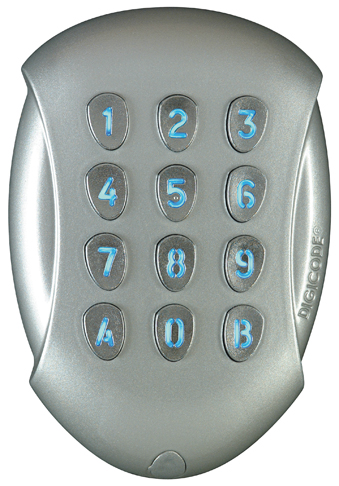
\includegraphics[width=.7\textwidth]{images/digicode}
%
%\textit{Digicode}
%\end{center}
%\end{minipage}\hfill
%\begin{minipage}[c]{.2\linewidth}
%\begin{center}
%%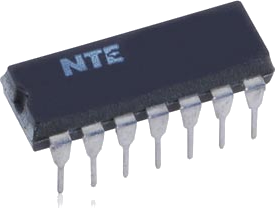
\includegraphics[width=.8\textwidth]{images/transistor_ttl_nand}
%
%\textit{Transistor TTL (permettant de réaliser des opérations logiques) }
%\end{center}
%\end{minipage}\hfill
%\begin{minipage}[c]{.2\linewidth}
%\begin{center}
%%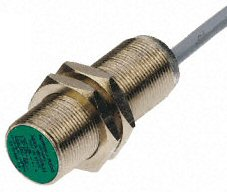
\includegraphics[width=.8\textwidth]{images/inductif}
%
%\textit{Détecteur inductif}
%\end{center}
%\end{minipage}\hfill
%\begin{minipage}[c]{.2\linewidth}
%\begin{center}
%%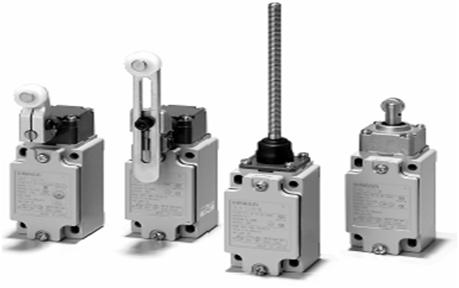
\includegraphics[width=\textwidth]{images/capteur_contact}
%
%\textit{Détecteur à contact}
%\end{center}
%\end{minipage}
%
%Un des objectifs de l'automaticien est de concevoir la partie commande qui traite les informations et élabore les ordres. Ce cours étudie le cas où les informations et les ordres élaborés sont des variables binaires.

\begin{center}
D'après les Sciences de l'Ingéneur en PTSI -- Éditions Ellipses

Laurent Deschamps \& Patrick Beynet
\end{center}

\begin{obj}
\begin{itemize}
\item Les différentes topologies et classification en fonction des distances couvertes.
\item Les sens possibles de transfert, simultané ou alterné.
\item L’absence ou la présence de synchronisation d’horloge entre les différents nœuds.
\item Les principaux médiums avec leurs caractéristiques.
\item Les différents mécanismes de gestion de conflit.
\item Le modèle OSI.
\end{itemize}
\end{obj}

\begin{savoir}
\textsc{Savoirs :}
\begin{itemize}
\item \textbf{Mod - C5.1 :} %Modélisation des systèmes à événements discrets (fonctions logiques, tables de vérité).
\end{itemize}
\end{savoir}

%\newpage 

\setlength{\parskip}{0ex plus 0.2ex minus 0ex}
 \renewcommand{\contentsname}{}
 \renewcommand{\baselinestretch}{1}

\tableofcontents

 \renewcommand{\baselinestretch}{1.2}
\setlength{\parskip}{2ex plus 0.5ex minus 0.2ex}

% \vspace{1cm}
\textit{Ce document évolue. Merci de signaler toutes erreurs ou coquilles.}

\section{Caractérisation d'un réseau}
\subsection{Classification, dimension}

\begin{itemize}
\item \textbf{LAN} : Local Area Network. Réseau de taille locale qui permet d’interconnecter des clients du réseau d’une entreprise : de quelques mètres à un kilomètre.
\item \textbf{MAN} : Metropolitan Area Network. Permet d’interconnecter plusieurs LAN géographiquement proches (au maximum quelques dizaines de km) à des débits importants.
\item \textbf{WAN} : Wide Area Network. Réseau de la taille d’une région à la terre. Permet à tous les LAN ou MAN de communiquer entre eux.
\end{itemize}

\subsection{Les différentes topologies}

\subsubsection*{Topologie en étoile}
\begin{minipage}[c]{.66\linewidth}
Un commutateur (switch) permet de connecter les équipements. Une machine perturbatrice, peut être isolée du réseau. Inconvénient : si le commutateur présente un défaut, tout le réseau est perturbé. C’est la structure actuelle d’un réseau Ethernet à paire torsadé (100 Base T, 1000 Base T).
\end{minipage} \hfill
\begin{minipage}[c]{.3\linewidth}
\begin{center}
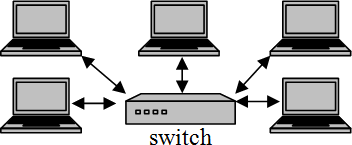
\includegraphics[width=.95\textwidth]{images/fig_01}
\end{center}
\end{minipage} 

\subsubsection*{Topologie de type bus}
\begin{minipage}[c]{.66\linewidth}
 Tous les équipements partagent une même liaison. Avantage : peu coûteux à mettre en œuvre. Inconvénient : la coupure du bus ou un élément perturbateur pénalise tout le  réseau (10 Base 5, CAN, I2C).
\end{minipage} \hfill
\begin{minipage}[c]{.3\linewidth}
\begin{center}
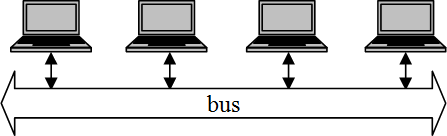
\includegraphics[width=.95\textwidth]{images/fig_02}
\end{center}
\end{minipage} 

\subsubsection*{Réseau en anneau}
\begin{minipage}[c]{.66\linewidth}
Chaque équipement possède un temps de parole sur le réseau. Les équipements sont connectés à un concentrateur (Toking Ring) ou en bus. Une carte « maître » fixe les temps de parole. On peut représenter ce fonctionnement par un « jeton » qui passe successivement dans chaque équipement (e.g. Interbus).
\end{minipage} \hfill
\begin{minipage}[c]{.3\linewidth}
\begin{center}
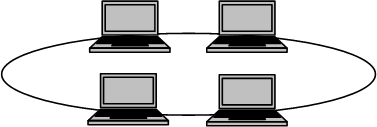
\includegraphics[width=.95\textwidth]{images/fig_03}
\end{center}
\end{minipage} 

\subsubsection*{Topologie maillée}

\begin{minipage}[c]{.66\linewidth}
Utilisés principalement par Internet, les réseaux maillés utilisent plusieurs chemins de transferts entre les différents nœuds. Des routeurs possèdent des tables de routages. Ils déterminent en temps réel le meilleur trajet parmi tous ceux possibles. Cette méthode garantit le transfert des données en cas de panne d'un nœud ou d’une liaison saturée qui  peut alors être assuré sur une autre liaison. Cette architecture est complexe à mettre en œuvre et n’est généralement pas utilisée dans les réseaux locaux.
\end{minipage} \hfill
\begin{minipage}[c]{.3\linewidth}
\begin{center}
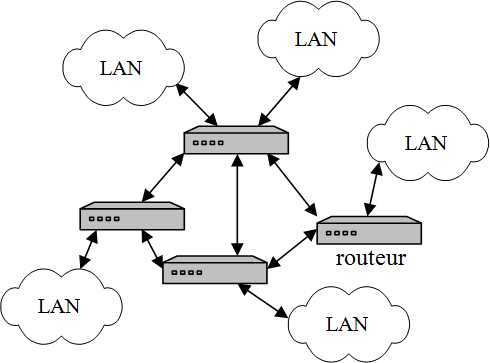
\includegraphics[width=.95\textwidth]{images/fig_04}
\end{center}
\end{minipage} 

\subsection{Quantités d’informations / Temps d’obtention}
Dans le cas de capteurs reliés à un calculateur, des informations de un bit à quelques octets sont échangées. Le temps de latence est relativement faible, quelques millisecondes. Inversement, l’obtention de plusieurs méga octets (texte, image, vidéo) peut mettre plus de temps. La conception d’un réseau est souvent un compromis entre ces deux critères : quantité et temps.
Le débit caractérise le rapport de ces deux dernières grandeurs. Il s’exprime de trois façons :
\begin{itemize}
\item en bits/s : nombre d’informations logiques par seconde;
\item en bauds (Bd) : nombre de symboles par seconde;
\item en hertz (Hz) : bande passante pour que la transmission des données soit fiable.
\end{itemize}

\subsection{Robustesse d'un réseau}

La robustesse vise à évaluer la capacité du réseau à continuer de fonctionner sous l’effet d’éléments perturbateurs internes ou externes.
Citons quelques exemples de perturbations possibles :
\begin{itemize}
\item perturbations électromagnétiques engendrant des états non désirés sur les fils de connexions;
\item débit important monopolisant l’accès au médium (support physique véhiculant les données);
\item « collisions » de données échangées;
\item nombre de nœuds connectés trop important voulant accéder au réseau.
\end{itemize}
Chacun des réseaux, à travers le médium et/ou les protocoles, apporte une solution à ces perturbations de façons à améliorer la robustesse.
Une méthode couramment utilisée est le contrôle de l’intégrité d’un message par le calcul d’un CRC (Cyclic Redundancy Check : contrôle de redondance cyclique) ou d’un checksum (somme de contrôle). L’émetteur envoie sa trame incluant un champ contenant le code d’intégrité qu’il a calculé. Le récepteur en fait de même et valide ou non la trame reçue. On note aussi le contrôle par bit de parité sur la liaison RS232 par exemple.


\subsection{Circulation des informations}

L’information peut circuler de différentes manières :
\begin{itemize}
\item dans un seul sens : liaison monodirectionnelle (émission Radio et TV, « broadcast » sur Internet);
\item dans les deux sens mais pas en même temps : half-duplex (Talkie Walkie, CB);
\item dans les deux sens et en même temps : full-duplex (téléphonie, Ethernet).
\end{itemize}

Le caractère half-duplex du Talkie Walkie est dû à l’utilisation d’une unique fréquence pour l’émission et la réception (et du fait que plus de deux équipements peuvent communiquer). Il est envisageable, dans le cas d’une liaison point à point reliant deux machines, d’utiliser le principe de multiplexage pour créer deux sens de transfert simultanés, et rendre ainsi la liaison full-duplex.

\begin{minipage}[c]{.6\linewidth}
Le spectre ci-contre peut représenter par exemple celui de l’ADSL. Bien qu’une seule paire de fils raccorde l’abonné au central, une première porteuse permet le transport montant autour de la fréquence $f_1$ (voire plusieurs fréquences) et le transport descendant autour de $f_2$ (voir plusieurs).
\end{minipage} \hfill
\begin{minipage}[c]{.36\linewidth}
\begin{center}
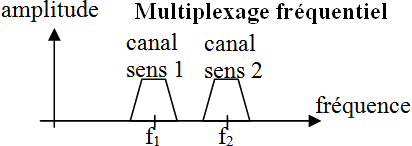
\includegraphics[width=.95\textwidth]{images/fig_05}
\end{center}
\end{minipage} 

\subsection{Mode de transmission}

\subsubsection*{La transmission série}
Une liaison série nécessite au moins deux fils (données sur un fil en half-duplex + un fil de masse), mais souvent trois : émission, réception et masse. Les bits sont transmis les uns à la suite des autres. A même médium, cette transmission sera plus robuste que la parallèle, moins chère (moins de connexions), mais n fois plus lente (n étant la largeur du mot).

\subsubsection*{La transmission parallèle}
Tous les bits du mot sont transmis simultanément sur $n$ fils.
Son coût dû au nombre de connexions, ainsi que son manque de robustesse la limite à une utilisation pour des courtes distances. Chaque canal ayant tendance à perturber les canaux adjacents, la qualité de la transmission se dégrade rapidement avec la vitesse et la longueur de la liaison. C’est une liaison qui est aujourd’hui  réservée aux très courtes distances.

\subsection{Synchronisation}

\subsubsection*{La transmission synchrone}
Dans la transmission série synchrone, les informations sont transmises de façon continue. Pour que cela soit possible, les horloges de l’émetteur et du récepteur doivent tendre à être identiques. Par contre, si les horloges sont asynchrones, bien que de même fréquence, une légère différence finit par décaler la lecture des mots. 

Il est impératif de dédier un fil pour la transmission de cette horloge.

Mais le plus souvent, un codage judicieux des niveaux logiques permet de transmettre l’information d’horloge mélangée à celles des données. Le récepteur, à l’aide d’une PLL (Phase Locked Loop), extrait la fréquence du signal émis, et lit en phase les bits (ou mots) transmis.
« Ethernet » est par exemple un bus synchrone. Soit grâce au code Manchester en 10 Mbits/s, soit avec les codage MLT-3 et 4B/5B en 100 Mbits/s.

\subsubsection*{La transmission asynchrone}

Dans la transmission série asynchrone, les informations ne sont pas transmises en continu. Ceci permet d’éviter tout décalage de lecture. Les horloges de l’émetteur et du récepteur sont de même fréquence, mais ne sont pas synchronisées.

Par exemple, des bits de synchronisation « Start » et « Stop » encadrent les informations de données dans le RS232. Ils ne servent pas à ce que les récepteurs asservissent leur horloge sur celle de l’émetteur, mais à ce qu’ils identifient bien le début des bits de données ; chaque horloge sera de fréquence presque identique, avec un glissement suffisamment faible pour lire tous les mots d’une trame avant un nouveau recalage.
Le codage des niveaux logiques peut permettre ou non de transporter en plus de l’information binaire, l’horloge.

\begin{minipage}[c]{.48\linewidth}
Si les bits ne subissent aucun codage :

\begin{center}
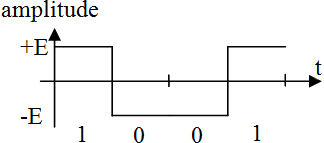
\includegraphics[width=.8\textwidth]{images/fig_06}
\end{center}

Les « 0 » sont à - 5 V et les « 1 » à 5 V.
On voit que si une longue série de mêmes bits est envoyée en continu, il devient difficile de savoir combien sont émis. L’information d’horloge ne pourrait être déduite que si un « 1 » puis un « 0 » étaient émis alternativement. C’est le principe de RS232, limité à l’envoi d’un octet entre deux conditions de « Start » et de « Stop ».


\end{minipage}  \hfill
\begin{minipage}[c]{.48\linewidth}
Selon le codage Manchester :

\begin{center}
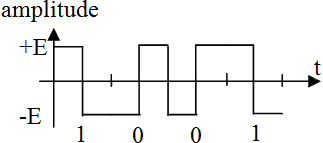
\includegraphics[width=.8\textwidth]{images/fig_07}
\end{center}

Les « 0 » sont codés par des fronts montants et les « 1 » par des fronts descendants.
Une longue série de mêmes bits va toujours produire des fronts, l’horloge réceptrice peut se synchroniser à l’aide de ces fronts.
Il nécessite d’avoir une bande passante deux fois plus grande que le signal d’origine car il y a deux états électriques sur la ligne pour un seul état logique.

\end{minipage} 

\subsection{Médium ou support physique}
Les supports physiques de transmission appelés aussi « médiums » influent sur :
\begin{itemize}
\item la vitesse de transmission,
\item la distance possible de transmission,
\item l'immunité aux perturbations électromagnétiques.
\end{itemize}

\subsubsection*{La paire de fils torsadés}
\begin{minipage}[c]{.78\linewidth}
Simple à mettre en œuvre, peu coûteuse et très répandue (réseau Ethernet, réseau téléphonique), sa bande passante est de l’ordre de la centaine de mégahertz.
\end{minipage} \hfill
\begin{minipage}[c]{.2\linewidth}
\begin{center}
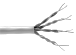
\includegraphics[width=.95\textwidth]{images/fig_08}
\end{center}
\end{minipage} 

\subsubsection*{Le câble coaxial}
\begin{minipage}[c]{.78\linewidth}
Il est composé d’un conducteur central (âme), d’un isolant diélectrique, d’une tresse de blindage et d’une protection extérieure. Il possède une bonne immunité aux perturbations, et est adapté aux transmissions à grande vitesse grâce à sa bande passante de l’ordre du gigahertz. Utilisé pendant des années pour les liaisons à très grande distance, il est maintenant concurrencé par la fibre optique
\end{minipage} \hfill
\begin{minipage}[c]{.2\linewidth}
\begin{center}
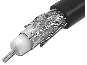
\includegraphics[width=.95\textwidth]{images/fig_09}
\end{center}
\end{minipage} 

\subsubsection*{La fibre optique}
\begin{minipage}[c]{.78\linewidth}
Elle ne conduit pas un signal électrique, mais un signal lumineux dans le cœur de la fibre qui peut-être en verre ou en plastique. Complètement insensible aux perturbations électromagnétiques et à faible perte, la fibre optique est particulièrement adaptée aux environnements industriels agressifs, et aux transmissions longues distances. Sa bande passante est de l’ordre de 50 GHz.
\end{minipage} \hfill
\begin{minipage}[c]{.2\linewidth}
\begin{center}
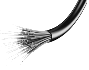
\includegraphics[width=.95\textwidth]{images/fig_10}
\end{center}
\end{minipage} 

\subsubsection*{Les liaisons électromagnétiques non guidées}
\begin{minipage}[c]{.78\linewidth}
Elles sont la base des récepteurs/émetteurs nomades. Les ondes électromagnétiques ont l’avantage de plutôt bien se propager dans le médium gratuit et immédiatement disponible qui est l’air. Cependant, elles sont soumises à de nombreuses normes en fréquence et en puissance d’émission, et ne sont pas à l’abri de perturbations extérieures difficiles à anticiper.
\end{minipage} \hfill
\begin{minipage}[c]{.2\linewidth}
\begin{center}
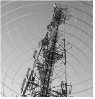
\includegraphics[width=.95\textwidth]{images/fig_11}
\end{center}
\end{minipage} 

\subsection{Techniques de transmission}
En fonction du médium, de ses possibilités, ainsi que du besoin de l’utilisateur, on peut utiliser trois techniques de transmission :
\begin{itemize}
\item la bande de base : aucune modification ou presque du signal. On envoie les bits tels quels sur le support (CAN, I2C, Ethernet, etc.),
\item la transposition de fréquence : le signal de données est placé autour d’une porteuse mieux adaptée au support ou aux plus longues distances (la voix via le Talkie Walkie),
\item le multiplexage temporel ou fréquentiel : cas du téléphone commuté, de l’ADSL, de la radio ou de la télévision. On profite d’une bande passante large ou d’une rapidité de transmission, pour faire passer plusieurs informations sur le médium.
\end{itemize}


\subsection{Les accès au médium}
Relier deux équipements et gérer l’absence de collision sur l’accès au médium, se fait sans trop de difficultés. Lorsque le nombre de matériels reliés augmente, il faut trouver un moyen d’arbitrer l’accès au médium.

\subsubsection*{Le principe « Maître / Esclave »}
Un élément, appelé maître, arbitre les esclaves qui peuvent accéder au support lorsque le maître les y autorisent. 

Ce principe est très efficace si seul le maître a besoin de décider quand il va donner l’accès. Si un des esclaves a besoin de se manifester sur un événement extérieur, il doit attendre l’autorisation du maître. Ceci crée un temps de latence. De la même manière, le maître passe son temps à donner un temps de parole aux esclaves susceptibles d’informer d’évènements extérieurs même en leur absence (« polling »), ce qui fait perdre du temps.

L’I2C est basé sur le principe maître-esclave. Il est bien adapté aux applications audio et vidéo. En effet, dans ces dernières, le microcontrôleur (maître) passe plus de temps à diriger les esclaves, qu’à les scruter pour attendre un événement.


\subsubsection*{Le principe de détection de collision (CSMA : Carrier Sense Multiple Access)}
Il consiste à autoriser tous les équipements raccordés au bus à prendre la parole dès qu’ils en ont besoin et que le bus est libre Tous les équipements ont le même niveau de priorité d’accès au médium. Il faut ensuite arbitrer si une collision survient après que deux équipements aient pris la parole au même moment. 

Le CSMA/CD (Collision Detect) consiste à détecter la collision : le premier équipement qui détecte le conflit arrête d’émettre et envoie un signal particulier pour prévenir les autres (cas de l’Ethernet).

Dans le cas du CSMA/CA (Collision Avoidance), bien que tous les équipements aient le même niveau d’accès au médium, celui qui possède un numéro d’identification plus prioritaire conservera l’accès au bus. Ceux qui le sont moins, le détecteront et cesseront d’émettre. Le plus prioritaire continuera l’émission de son message sans avoir besoin de recommencer. C’est le cas du bus CAN.

\subsection{Échanges d’informations sur le médium}
Les échanges d’informations peuvent se faire selon trois modes.

\subsubsection*{La liaison point à point}
La liaison point à point (P2P) est une liaison entre deux matériels uniquement.

\subsubsection*{Le mode client / serveur}
Le client demande des informations à une machine, le serveur. Ce dernier répond alors aux requêtes du client. Plusieurs matériels peuvent se connecter au serveur. Exemple : I2C ; un serveur WEB ou FTP, etc. Pour un client en mode connecté, cela peut être se ramener à une liaison point à point.

\subsubsection*{Le mode producteur / consommateur (diffusion)}
Un équipement diffuse une information, les consommateurs décident ou non d’utiliser cette information. Exemple : le bus CAN, la télévision ou la radio.

\subsection{Le modèle OSI}

\begin{minipage}[c]{.68\linewidth}
Afin de rationaliser le modèle des réseaux, l’Open Systems Interconnection (OSI) a défini sept couches permettant de spécifier chaque service nécessaire au fonctionnement d’un réseau.
\end{minipage} \hfill
\begin{minipage}[c]{.3\linewidth}
\begin{center}
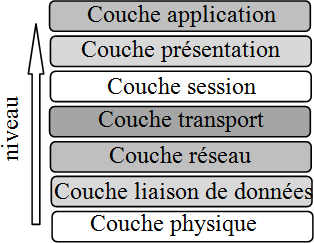
\includegraphics[width=.95\textwidth]{images/fig_12}
\end{center}
\end{minipage} 

Chacune d’entre-elles a une fonction bien définie, elle se sert de services, et en propose aux couches adjacentes : 
\begin{itemize}
\item la couche « physique » gère le codage des bits à transmettre en fonction du type de médium;
\item la couche « liaison de données » fractionne les données en trame et a pour fonction de présenter des données sans erreur à la couche réseau;
\item la couche « réseau » gère des paquets de données et assure le routage grâce à un adressage des matériels;
\item la couche « transport » est responsable de l’acheminement de bout en bout d’un paquet de données découpé en segments de taille dépendant du type de réseau;
\item la couche « session » synchronise les échanges entre tâches distantes. Elle fait le lien entre adresse logique (e.g. IP) et physique (e.g. MAC);
\item la couche « présentation » traite les informations pour les rendre compatibles avec la syntaxe définie;
\item la couche « application » est la partie visible pour l’utilisateur ; c’est elle qui propose les services de messagerie, internet, ftp, etc.
\end{itemize}

Le dialogue entre couches de même niveau de deux matériels connectés, nécessite l’utilisation de protocoles spécifiques.

\subsection{Positionnement des bus de données}
\begin{center}
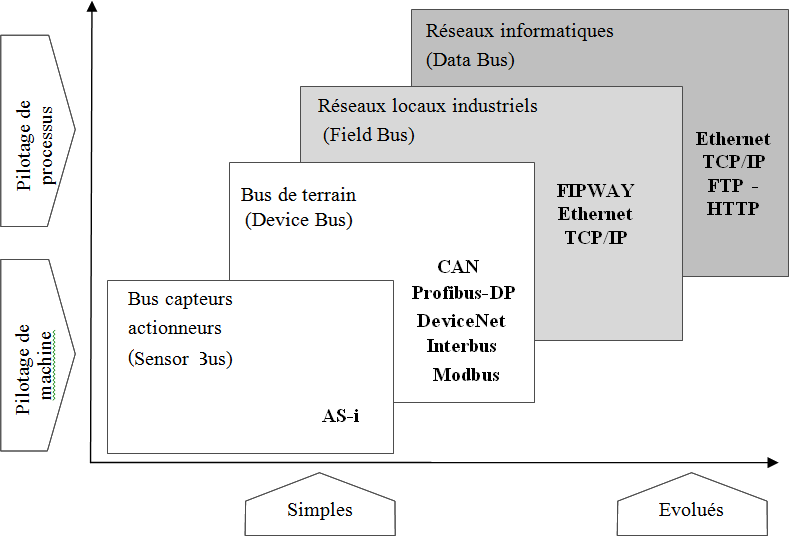
\includegraphics[width=.8\textwidth]{images/fig_13}
\end{center}


\section{Exemples de réseaux}
\subsection{Ethernet et le protocole TCP / IP}

Le modèle TCP / IP (Transmission Control Protocol / Internet Protocol), créé aux États Unis, bien qu’antérieur au modèle OSI, adopte une approche modulaire. Il est possible d’établir un parallèle entre les couches des deux modèles :
\begin{center}
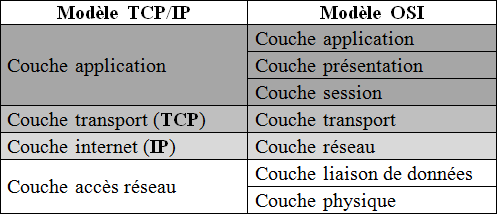
\includegraphics[width=.65\textwidth]{images/fig_14}
\end{center}

Le TCP/IP est un protocole à commutation de paquets. L’information est découpée en plusieurs morceaux qui sont réassemblés à l’arrivée. Le chemin pour aller de la source au destinataire n’est pas établi à l’avance (contrairement au réseau dit « commuté » où la liaison physique réservé est établie à l’avance entre le destinataire et l’émetteur) et peut emprunter plusieurs chemins (réseau maillé).

Les fonctions des différentes couches sont les suivantes : 
\begin{itemize}
\item couche « application » : englobe les applications standards du réseau (SMTP, FTP, HTTP, etc.);
\item couche « transport » : assure l'acheminement des données;
\item couche « internet » : fournit le paquet de données (datagramme);
\item couche « accès réseau » : spécifie la forme sous laquelle les données doivent être acheminées quel que soit le type de réseau utilisé (Ethernet, PPP, Wi-Fi, etc.).
\end{itemize}

\begin{center}
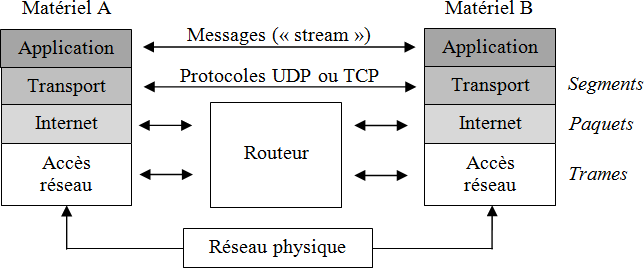
\includegraphics[width=.75\textwidth]{images/fig_15}
\end{center}

\subsubsection*{Quelques protocoles « application »}
\begin{itemize}
\item HTTP : protocole utilisé pour les serveurs web;
\item FTP : protocole pour l’échange de fichiers;
\item SMTP : protocole pour l’échange d’e-mail;
\item DNS : Permet d’obtenir une adresse IP routable correspondant à un nom de serveur.
\end{itemize}

\subsubsection*{Les deux protocoles de « transport »}
\begin{itemize}
\item UDP : échange de segments sans accusé de réception des données. Il est non fiable.
\item TCP : plus fiable que l’UDP, il crée un mode connecté virtuel. Les en-têtes sont plus volumineux que ceux de l’UDP.
\end{itemize}

\subsubsection*{L’adressage IP}

L’IP (Internet Protocol) est un service de la couche « réseau », sans connexion et non fiable. Il est chargé d’acheminer les paquets à la bonne adresse, en utilisant le plus court chemin. On parle de routage de données.

L’adresse IP est une adresse logique « routable », donnée à chaque équipement connecté au réseau et susceptible de traiter des paquets IP. Elle permet avec son masque de définir un réseau logique, d’échanger entre deux machines (« unicast »), de diffuser à un groupe de machine (« multicast »), ou sur tout le réseau (« broadcast »).
Elle est composée de quatre octets (IPv4), séparés par un point. Par exemple : 192.168.0.1.

Ce protocole possède des services qui lui sont propres : 
\begin{itemize}
\item ARP : permet d’obtenir une adresse physique (MAC) à partir d’une adresse IP;
\item RARP : permet d’obtenir une adresse IP à partir d’une adresse MAC;
\item ICMP : permet de tester la couche IP et réseau (utilisé par la commande « ping »).
\end{itemize}

\subsubsection*{L’adressage MAC}
La couche « Accès réseau » est la couche où circulent physiquement les données sous formes de trames. Une adresse physique MAC (e.g. 08 - AB - 27 - 0C - 50 - 66) codée sur six octets, propre et unique au monde, est attribuée à chaque matériel accédant à l’Ethernet. Mais, le TCP/IP peut aussi utiliser le Wi-Fi (Wireless Fidelity) ou la paire téléphonique via le PPP (Point-to-Point Protocol) pour l’ADSL.

\subsubsection*{L’encapsulation}
Pour chaque protocole, un en-tête est ajouté. C’est le principe de l’encapsulation.
L’analyse d’une trame TCP/IP Ethernet montre l’en-tête Ethernet avec les adresses MAC, puis celui IP avec ses adresses, puis le TCP ou l’UDP.

Ainsi, pour une application travaillant selon TCP/IP sur Ethernet, obtient :

\begin{center}
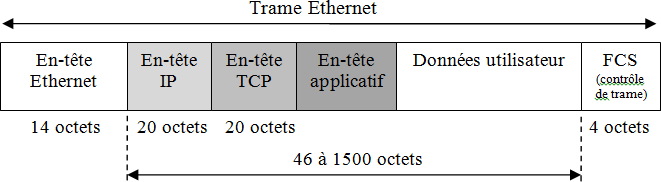
\includegraphics[width=.8\textwidth]{images/fig_16}
\end{center}

\subsubsection*{Le principe de détection de collision}
Le principe du CSMA/CD (collision destructive) est utilisé sur le bus Ethernet :
\begin{itemize}
\item détection de la collision;
\item arrêt de la transmission de la trame;
\item émission d’une trame de brouillage;
\item attente d’un temps aléatoire;
\item réémission de la trame.
\end{itemize}

\subsection{Le bus CAN}

Le bus CAN (Controller Area Network) a été développé par la société Bosch pour les besoins de l’automobile. Il ne comprend qu’une partie des deux premières couches (« physique » et « liaison de données ») du modèle OSI. Sa relative robustesse aux agressions électromagnétiques lui a ouvert d’autres milieux d’applications, industrielles par exemple.
Le médium le plus utilisé pour un bus CAN est une paire torsadée, mais cela n’est pas imposé par la norme.

Des terminaisons (résistance de 120 $\Omega$) sont disposées à chaque extrémité de bus pour éviter les effets réflectifs.

La paire torsadée est en mode différentiel, un fil s’appelle CAN-H (High) et l’autre CAN-L (Low). Ce mode effectue une soustraction entre les deux signaux, et permet d’éliminer un parasite qui serait commun à ceux-ci.

La structure de bus a été retenue avec des mécanismes permettant de prévenir les perturbations d’échange en cas de nœud défaillant.

La longueur maximale du bus est d’un kilomètre. Le débit peut aller de 10 kbits/s à 1 Mbits/s, pour une longueur de bus respectivement de 1 kilomètre à 25 mètres.

\begin{center}
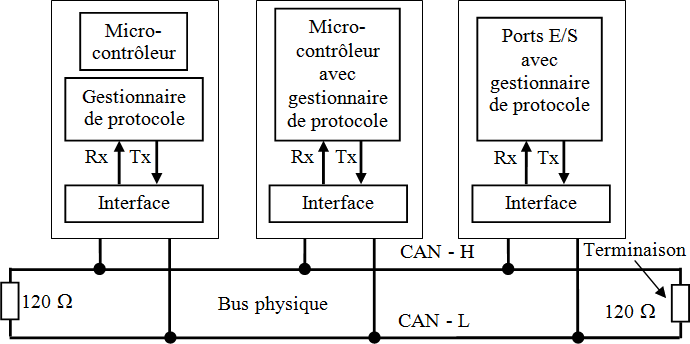
\includegraphics[width=.8\textwidth]{images/fig_17}
\end{center}


Il est possible de raccorder jusqu’à 128 nœuds sur le bus.
L’accès au médium se fait sur le principe de CSMA/CA, c'est-à-dire avec détection de conflit de prise de bus sans destruction de message. Cela est rendu possible grâce au principe des bits dominants (« 0 ») et récessifs (« 1 »). Lors de l’arbitrage, le premier champ après le bit Start Of Frame (SOF), contient l’identifiant du message. Donc, le message le plus important doit avoir le numéro d’identifiant le plus faible.

Chaque nœud vérifie que le bus est libre avant d’entamer une émission. Ensuite, à chaque fois qu’il transmet un bit, il relit l’état du bus pour voir s’il est réellement transmis. S’il impose un bit dominant, il relit bien cet état. Mais s’il émet un bit récessif et qu’un autre nœud lui impose un bit dominant, il comprend qu’il n’est plus prioritaire. Il cesse alors d’émettre.

\begin{center}
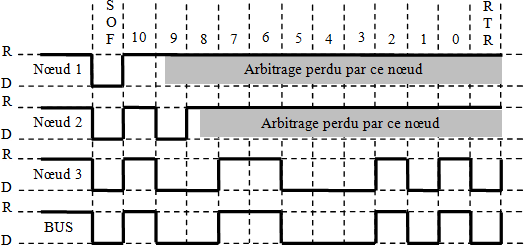
\includegraphics[width=.8\textwidth]{images/fig_18}
\end{center}

Contrairement à beaucoup de protocoles ou chaque équipement possède une adresse afin qu’un message puisse être envoyé à un nœud désigné, chaque nœud émet des messages avec son identifiant mais pas l’identifiant du destinataire. Ceci est rendu possible grâce au principe « producteur / consommateur ». Dans le cas du bus CAN, cet identifiant codé sur 11 bits, est situé en début de message. Il renseigne les récepteurs sur la nature des données contenues dans chaque message. Chaque récepteur décide ensuite de consommer ou non les données.

\subsubsection*{Chronogramme des signaux CAN-H et CAN-L}

\begin{minipage}[c]{.48\linewidth}
\begin{center}
CAN low speed (max. 125 kbits/s)

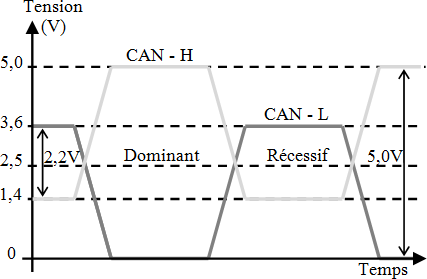
\includegraphics[width=.8\textwidth]{images/fig_19}
\end{center}
\end{minipage} \hfill 
\begin{minipage}[c]{.48\linewidth}
\begin{center}
Le CAN high speed (max. 1 Mbits/s)

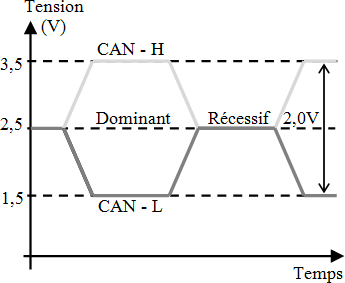
\includegraphics[width=.8\textwidth]{images/fig_20}
\end{center}
\end{minipage}

\subsection{L'I2C}
L’I2C est un bus développé par Philips au début des années 80 pour répondre au besoin croissant des échanges numériques dans l’électronique domestique, notamment dans les téléviseurs modernes : échange entre microcontrôleur, récepteur Infra Rouge, tuner, etc.
Il est composé de trois fils :
\begin{itemize}
\item un fil de donnée bidirectionnel SDA;
\item un fil d’horloge unidirectionnel SCL;
\item la référence de tension (Masse).
\end{itemize}
La vitesse de transmission va de 100 kbit/s à 5 Mbits/s (version 4 en 2012).
Comme le bus CAN, il existe des bits dominants (niveau logique « 0 ») et des bits récessifs (niveau logique « 1 »). Cependant, cette hiérarchisation des bits n’a d’intérêt que dans le cas de multi-maîtres.

Les maîtres imposent l’horloge aux périphériques qui n’ont pas leur propre horloge interne, il s’agit donc d’une liaison synchrone.
Le bus de données est unique et bidirectionnel. Les échanges ne se font que dans un seul sens à un instant donné, la liaison est donc en half-duplex.

C’est souvent un seul maître (microcontrôleur) qui interroge les périphériques. Nous sommes dans le principe du maître-esclave. Néanmoins, rien n’empêche d’avoir plusieurs maîtres, et un maître peut aussi par moment devenir esclave.

Chaque esclave doit posséder sa propre adresse. Le maître n’en a pas besoin. L’adresse est composée de huit bits. Le huitième bit précise à l’esclave si le maître veut faire une procédure de lecture (bit à « 1 ») ou une écriture (bit à « 0 »). Les adresses des composants (sept premiers bits) sont fixées en usine pour certains. Pour d’autres, susceptibles d’être utilisés en nombre sur une carte, une partie est fixée en usine, et l’autre est configurable par trois broches sur le composant. 

\begin{center}
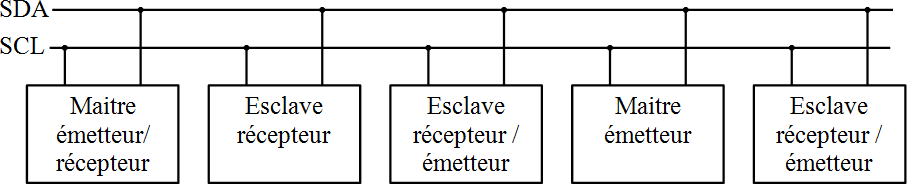
\includegraphics[width=.8\textwidth]{images/fig_21}
\end{center}

Pour utiliser le bus et interroger un esclave :
\begin{itemize}
\item le maître doit vérifier que le bus est libre (SDA et SCL à « 1 »),
\item émettre une condition de « Start » (SDA passe à « 0 » alors que SCL est toujours à « 1 »),
\item envoyer les sept bits d’adresse et ajouter le 8ème pour une lecture ou écriture,
\item l’esclave précise qu’il a reconnu son adresse et émet un bit d’acquittement.
\end{itemize}

Si par exemple il s’agit d’une demande de lecture, le maître va continuer d’envoyer un signal d’horloge, mais c’est l’esclave qui va imposer les états sur le bus de données. 
Pour finir un échange et libérer le bus, une condition de « Stop » doit être émise (SDA passe à « 1 » alors que SCL toujours à « 1 »).

Pour envoyer un bit, celui-ci doit être stable durant le temps ou SCL est à « 1 » (variation de SDA interdit durant cette période) et peut changer d’état quand SCL est à « 0 ».

\begin{center}
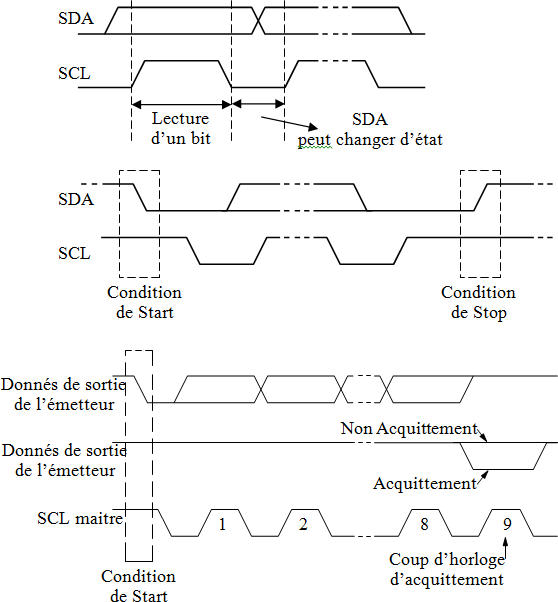
\includegraphics[width=.8\textwidth]{images/fig_22}
\end{center}

\subsection{Mais encore...}

On notera bien d’autres exemples de réseaux très utilisés : téléphonies fixe et mobile, LAN sans fil (Wi-Fi), RFID (Radio Frequency Identification pour les réseaux sans fil de capteurs), etc.
 

\section{Méthodes -- Comment déterminer les caractéristiques d’un réseau ?}
\subsection{Détermination des éléments physiques d’un réseau}

L’étude d’un réseau peut commencer par l’étude de la partie physique du réseau. Le but est de déterminer la longueur maximale de la liaison afin de déterminer si c’est un LAN, un WAN ou un MAN. La connexion entre les équipements va nous guider sur la topologie (bus, étoile). Mais celle-ci ne doit pas être confondue avec l’aspect physique. Par exemple, le 10BaseT branché sur un Hub ressemble à une topologie étoile, c’est pourtant une connexion de type Bus. Le Token Ring (topologie en anneau) lui aussi passe par un concentrateur qui ferait penser à une topologie en étoile. Pour finir, le type de médium sera à déterminer, et aidera à connaître le type de liaison : série ou parallèle. Toutes ces informations sont à extraire des schémas et du texte présentant le réseau.

\begin{exemple}
\textit{Bus de terrain MVB pour réseau ferroviaire}
\end{exemple}

Les informations devant être transmises par l’intermédiaire du bus MVB (Multifunction Vehicule Bus) sont codifiées par les unités électroniques locales (EDCU, climatisation, pantographe, etc.) qui sont branchées sur le bus.

\begin{center}
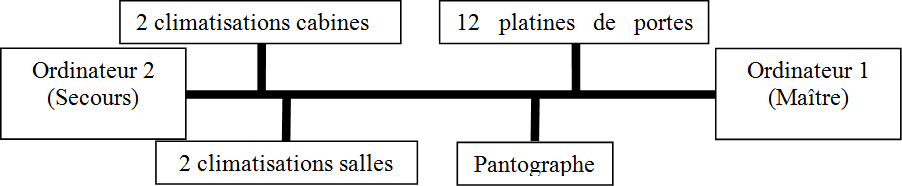
\includegraphics[width=.8\textwidth]{images/fig_23}
\end{center}

La norme IEC indique que ce protocole peut être utilisé sur une paire torsadée ou sur une fibre optique pour former un bus.
La vitesse du bus est de 1,5 Mbits/s, avec un temps de réponse d’environ 10 µs. 
Le bus peut couvrir des distances jusqu’à 2 km, découpées en portion de 200 m et de 20 m.

\begin{center}
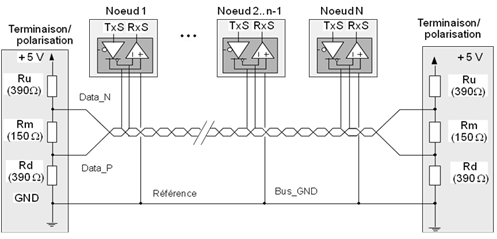
\includegraphics[width=.8\textwidth]{images/fig_24}
\end{center}

Ce que nous indique la lecture de la présentation de cette norme :
La lecture des informations nous indique que la longueur de bus dans sa spécification ne dépasse pas les 2 km. Il fait donc partie des réseaux type LAN, plus souvent appelé bus de terrain pour ce type d’application.

Le médium supporté par la norme peut-être une paire torsadée, ou une fibre optique. Dans l’image du bus ci-dessus, on voit la représentation de la paire torsadée en mode différentiel. Ces deux supports présentent une bonne immunité aux perturbations électromagnétiques.
Chaque nœud se connecte sur le médium commun à tous les nœuds et voit tout le trafic : nous avons donc une structure de bus.

Nous avons ici affaire à une paire torsadée, c’est donc une liaison série.

\subsection{Détermination du type de liaison dans un réseau}
Une fois la partie physique déterminée, il faut connaître la manière avec laquelle les équipements vont accéder aux réseaux.
La liaison est-elle synchrone ou asynchrone ?
Dans quel sens peuvent circuler les informations, simultanément ou non ?
Comment est géré l’accès au bus et quelle stratégie est adoptée en cas de collision ?

\begin{exemple}
Bus de terrain MVB pour réseau ferroviaire
\end{exemple}

Le protocole utilisé définit la procédure d’établissement de connexion, le transfert du message, la fin de la connexion entre le maître (ordinateur) et les esclaves (unités électroniques indépendantes). Le maître interroge un des esclaves, et il attend sa réponse. 
Chaque élément raccordé sur le bus possède une adresse de 12 bits. Pour les platines de portes, les huit bits de poids fort sont figés et les quatre bits de poids faible sont paramétrables par la mise en place de cavaliers sur les cartes électroniques ECDU. Les bits sont transférés selon le principe du code Manchester. 

En cas de réponses multiples, la collision est détectée par le maître. Une procédure d’interrogation par parité d’adresse est prévue dans la norme.


Ce que nous indique la lecture de la présentation de cette norme :

Le principe du « maître / esclave » est appliqué, arbitrant normalement l’utilisation du bus. Néanmoins, le principe de CSMA/CD est prévu dans la norme.
Les bits sont émis sur le bus selon le codage de ligne Manchester, la liaison pourra être synchrone.

Pour finir, chaque nœud se connecte au bus seulement avec deux fils et émet sur le bus à l’aide d’un simple driver (porte amplificatrice de niveau logique et de son complément). Tout indique qu’aucun multiplexage n’est effectué ; à un instant donné, un seul nœud prend le contrôle du bus et tous les autres doivent écouter : il s’agit d’une liaison half-duplex.

\subsection{Détermination de la structure des données}
Une fois établie la manière dont les nœuds peuvent communiquer sur le bus, il reste à déterminer comment les données vont être organisées. 
Il faut que le ou les destinataires sachent que la trame est pour eux, et qu’ils puissent en extraire les données utiles.

\begin{exemple}
Bus de terrain MVB pour réseau ferroviaire
\end{exemple}

Le maître envoie sur le bus le message de 33 bits suivant :

\begin{center}
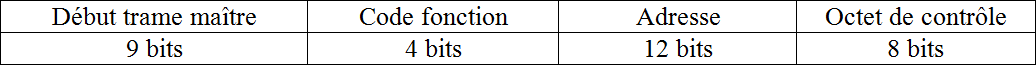
\includegraphics[width=.95\textwidth]{images/fig_25}
\end{center}

%\begin{center}
%\begin{tabular}{|c|c|c|c|}
%\end{tabular}
%\end{center}

L'esclave concerné répond alors sur le bus le message de 33 bits suivant :

%\begin{center}
%\begin{tabular}{|c|c|c|}
%\end{tabular}
%\end{center}

\begin{center}
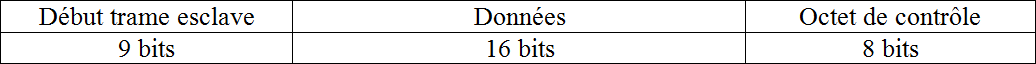
\includegraphics[width=.95\textwidth]{images/fig_26}
\end{center}

Les messages se terminent par un signal électrique spécifique (ED : End delimiter).
L'émetteur du message génère l'octet de contrôle avec un algorithme spécifique. Celui qui reçoit le message effectue la même opération et peut ainsi vérifier s’il n'y a pas eu d'erreur de transmission.

La lecture des informations logiques présentes sur les cartes ECDU se fait avec le code fonction.
Exemple d'informations logiques présentes sur les cartes ECDU (codés sur 33 bits) :

\begin{center}
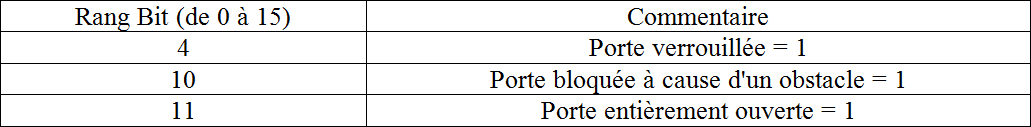
\includegraphics[width=.95\textwidth]{images/fig_27}
\end{center}

%\begin{center}
%\begin{tabular}{|c|c|}
%\end{tabular}
%\end{center}

Exemple d'échange : le maître désire connaître l'état de la porte 5 :

\begin{center}
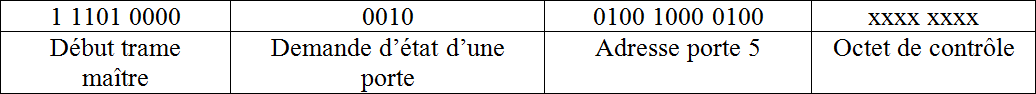
\includegraphics[width=.95\textwidth]{images/fig_28}
\end{center}

%\begin{center}
%\begin{tabular}{|c|c|c|c|}
%\end{tabular}
%\end{center}

L'esclave répond

\begin{center}
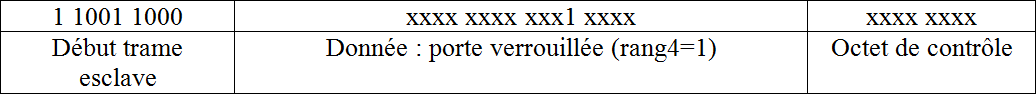
\includegraphics[width=.95\textwidth]{images/fig_29}
\end{center}
%\begin{center}
%\begin{tabular}{|c|c|c|c|}
%\end{tabular}
%\end{center}

Ce que nous indique la lecture de la présentation de cette norme :
Un en-tête en début de message permet de distinguer s’il provient du maître (requête) ou d’un esclave (réponse).
On voit qu’un message émanant du maître possède l’adresse de l’esclave destinataire.
Par contre, quand l’esclave répond, il n’y a aucune adresse. Elle est inutile car après la requête, le maître sait que le message émis, est la réponse de l’esclave qu’il vient d’interroger.
Le maître dispose de quatre bits pour formuler une requête à un esclave. Il y a donc seize demandes différentes possibles. L’exemple donné est le quartet « 0010 » qui est la demande de l’état d’une porte. L’esclave possède seize bits pour répondre à la requête, par exemple le 4ème bit indique si la porte est verrouillée ou non.
La fin de trame est constituée d’un octet de contrôle, type CRC, afin de vérifier l’intégrité du message.


\begin{thebibliography}{2}
%\bibitem{dv}{Supports de cours de David Violeau, Lycée Saint-Louis, Paris.}
%\bibitem{sg}{Stéphane Genouël, \textit{Systèmes Séquentiels -- Fonction mémoire}, Cours de MPSI -- PCSI, Lycée Chateaubriand, Rennes, \url{http://stephane.genouel.free.fr/}.} 
\bibitem{pb}{Laurent Deschamps, Patrick Beynet et Al., \textit{Sciences Industrielles pour l'Ingénieur, PTSI}, Éditions Ellipses, à paraître.}
%\bibitem{3}{Pierre Debout, \textit{Automatique -- Systèmes à événements discrets}, Cours de PCSI.}
%\bibitem{4}{Thierry Schanen, \textit{Guide des automatismes 9.1}, Pos Industry, 2009.}
%\bibitem{fm}{Supports de cours de Florestan Mathurin, Lycée Bellevue, Toulouse.}
%\bibitem{jpp}{Supports de cours de Jean-Pierre Pupier, Lycée Rouvière, Toulon}

\end{thebibliography}

\end{document}\end{document}


